\documentclass{article}
\usepackage[utf8]{inputenc}
\usepackage[margin=1.2in]{geometry}
\usepackage{hyperref}
\usepackage{listings}
\usepackage{xcolor}
\usepackage{natbib}
\usepackage{graphicx}
\usepackage{amsmath}

\title{\vspace{-2 cm}Universidade Federal de Ouro Preto \\ BCC502 - Metodologia Científica para Ciência da Computação \\\textbf{ Observaçõe como intervenção Prática}}
\author{Prof. Rodrigo Silva}
\date{}


\begin{document}

\maketitle

\section{Anteriormente}

\begin{enumerate}
    \item O conhecimento científico tem um status especial em parte porque é baseado em uma base segura , fatos sólidos firmemente estabelecidos por observação.
    \item Problemas
    \begin{enumerate}
        \item Percepções são influenciadas pela experiência e expectativas do observador
        \item Julgamento sobre a veracidade da descrição da observação depende do que já se sable 
        \item Assim fatos observáveis são tão falíveis (sucepstíveis a erro) quanto as pressuposições que os sustentam.    
    \end{enumerate}
\end{enumerate}

\section{Observção como intervenção prática}

\begin{enumerate}
    \item 
\end{enumerate}

\begin{figure}[!htbp]
    \centering
    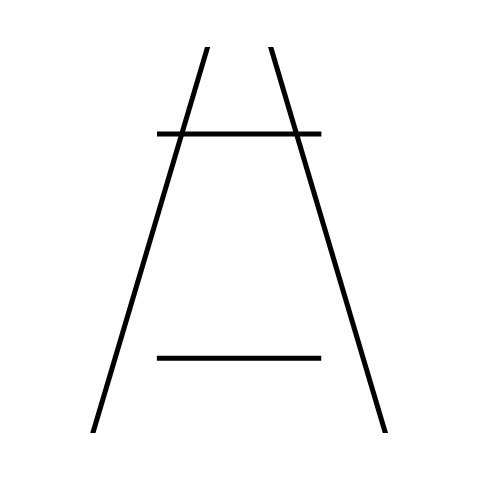
\includegraphics[width=0.3\textwidth]{Ponzo_Illusion.png}
    \caption{Illusion}
    \label{fig:illusion1}
\end{figure}

\begin{figure}[!htbp]
    \centering
    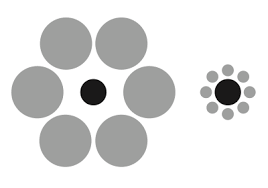
\includegraphics[width=0.4\textwidth]{ilusao_ebin.png}
    \caption{Illusion}
    \label{fig:illusion2}
\end{figure}

\section*{Fonte}

\begin{itemize}
    \item Chalmers, Alan F. What is this thing called science?. Hackett Publishing, 2013.
\end{itemize}

%\bibliographystyle{plain}
%\bibliography{references}
\end{document}

